%        File: DesignDocument.tex
%     Created: 一 3月 26 01:00 下午 2018 C
% Last Change: 一 3月 26 01:00 下午 2018 C
%
\documentclass[UTF8,noindent]{ctexart}
\usepackage[a4paper,left=2.0cm,right=2.0cm,top=2.0cm,bottom=2.0cm]{geometry}
\usepackage{hyperref}
\usepackage{url}
\usepackage{graphicx}
\usepackage{amsmath}
\usepackage{amssymb}
\usepackage{enumitem}
\usepackage{tikz}
\usepackage{float}
\usepackage{xeCJK}
\usepackage{listings}
\usepackage{xcolor}
\lstset{language = c,numbers=left, showstringspaces=false,keywordstyle= \color{ blue!70 },commentstyle=\color{red!50!green!50!blue!50}, frame=shadowbox, rulesepcolor= \color{ red!20!green!20!blue!20 } 
} 
\CTEXsetup[format={\Large\bfseries}]{section}
\usetikzlibrary{graphs}
%\newtheorem*{lemma}{Lemma}
\title{\CJKfamily{zhkai}计算机网络研讨课实验报告}
\author{{\CJKfamily{zhkai}冯吕}\ $2015K8009929049$}
\date{\today}
\begin{document}
\maketitle
\zihao{5}
\CJKfamily{zhsong}
%\begin{center}
%  \begin{tabular}{|p{15cm}|}
%    \hline
\section*{{\CJKfamily{zhhei}实验题目}}生成树机制实验
%\hline
\section*{{\CJKfamily{zhhei}实验内容}}
在本次实验中,需要基于已有代码,实现生成树运行机制,主要需要实现端口收到$config$包以后需要进行的操作,然后对于给定拓扑,计算输出相应状态下的最小生成树拓扑。

另外,需要自己构造一个不少于六个节点,链路冗余度不少于$2$的拓扑,然后使用$stp$程序计算输出最小生成树拓扑。
\section*{{\CJKfamily{zhhei}实验流程}}

\subsection*{处理$config$消息}
在实验过程中,首先在已有代码基础上实现生成树运行机制,即实现函数$static\ void\ stp\_handle\_config\_packet(stp\_t\ *stp,\ stp\_port\_t\ *p, struct\ stp\_config\ *config)$,该函数的功能是当$stp$节点从端口$p$收到$config$包以后的消息处理操作。

根据生成树机制,在初始化时,每一个节点都把自己当成根节点,将每个端口都设置为指定端口。当一个端口收到$config$消息之后,首先比较本端口存储的$config$和收到的$config$的优先级高低,比较规则如下图所示:
\begin{figure}[H]
  \centering
  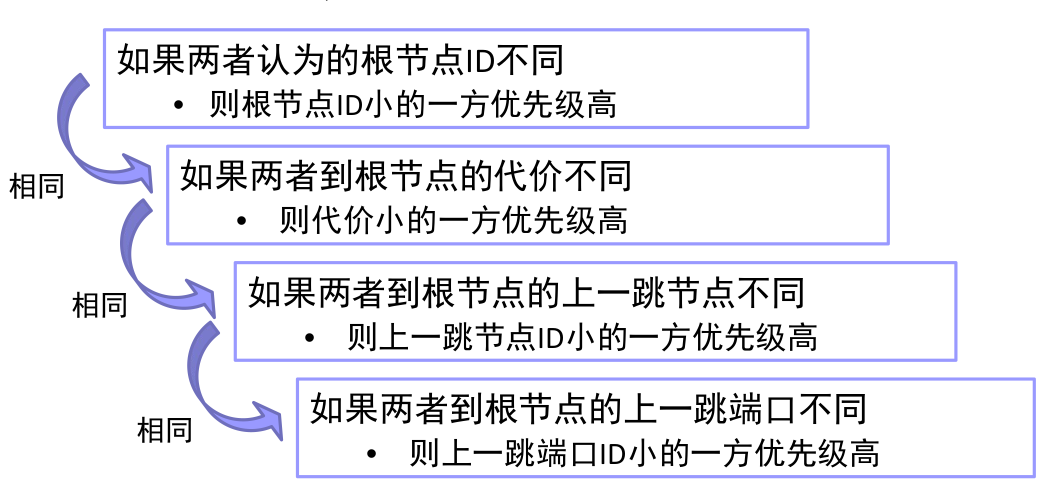
\includegraphics[scale=0.3]{cmp.png}
\end{figure}
由于比较逻辑较为复杂,因此,可通过定义如下宏定义来简化优先级比较:
\begin{lstlisting}
#define PRIOR(r1, r2, c1, c2, s1, s2, p1, p2) \
      r1<r2|| \
     (r1==r2&&c1<c2)|| \
     (r1==r2&&c1==c2&&s1<s2)|| \
     (r1==r2&&c1==c2&&s1==s2&&p1<p2)
\end{lstlisting}

比较完优先级之后,如果发现收到的$config$消息优先级高,那么说明该网段通过对方端口连接根节点代价更小,则将本端口存储的$config$替换为收到的$config$,本端口从指定端口变为非指定端口:
\begin{lstlisting}
if (PRIOR(ntohll(config->root_id),p->designated_root,
    ntohl(config->root_path_cost), p->designated_cost,
    ntohll(config->switch_id), p->designated_switch,
    ntohs(config->port_id), p->designated_port))
{
     //update port config
     p->designated_root = ntohll(config->root_id);
     p->designated_port = ntohs(config->port_id);
     p->designated_switch = ntohll(config->switch_id);
     p->designated_cost = ntohl(config->root_path_cost);
	 . . .
}
\end{lstlisting}

然后,更新节点状态。更新节点状态时,首先需要找出根端口,根端口需要满足两个条件:必须是非指定端口,且该端口的优先级需要高于其他所有的非指定端口。寻找根端口的代码如下:
\begin{lstlisting}
char not_de_port[stp->nports];
for(int i = 0; i != stp->nports; ++i){
    if (!stp_port_is_designated(&stp->ports[i]))
       not_de_port[i] = 1;
    else
        not_de_port[i] = 0;                                                                                                                     
}
stp_port_t *root_port = NULL;
for (int i = 0; i != stp->nports; ++i){
    if (not_de_port[i] && !strcmp(stp_port_state(&stp->ports[i]), 
	                "ALTERNATE")){
       root_port = &stp->ports[i];
       break;
    }
 }
 for (int i = 1; i != stp->nports; ++i){
     if ( !root_port ){// root port not exist, 
        //this switch is root switch
        stp->designated_root = stp->switch_id;
        stp->root_path_cost = 0;
        break;
     }
     if (not_de_port[i]&&!strcmp(stp_port_state(&stp->ports[i]),
          "ALTERNATE")&&(PRIOR(stp->ports[i].designated_root, 
          root_port->designated_root, stp->ports[i].designated_cost,
          root_port->designated_cost, stp->ports[i].designated_switch,
          root_port->designated_switch, stp->ports[i].designated_port,
          root_port->designated_port)))
        root_port = &stp->ports[i];
}
\end{lstlisting}

在寻找根端口的过程中,有判断根端口不存在的逻辑,如果不存在根端口,则说明该节点为根节点,需要将节点的$designated\_root$设置为节点$id$,并将$root\_path\_cost$设置为$0$(见上面代码第$19,20$行)。

如果根端口存在,那么选择通过$root\_port$连接到根节点,并如下更新节点状态:
\begin{lstlisting}
if (root_port){
    stp->designated_root = root_port->designated_root;
    stp->root_port = root_port;
    stp->root_path_cost = root_port->designated_cost + root_port->path_cost;
}
\end{lstlisting}

当节点更新完状态之后,还需要更新端口的$config$:
\begin{itemize}
  \item 如果一个端口是指定端口,那么只需更新如下内容:
\begin{lstlisting}
if (stp_port_is_designated(&stp->ports[i])){
    stp->ports[i].designated_root = stp->designated_root;
    stp->ports[i].designated_cost = stp->root_path_cost;
}
\end{lstlisting}
\item 如果一个端口为非指定端口,且其网段通过本节点到根节点的代
价比通过对端节点的代价小,那么该端口成为指定端口,并如下更新:
\begin{lstlisting}
if (!strcmp("ALTERNATE",stp_port_state(&stp->ports[i]))
    &&stp->root_path_cost < stp->ports[i].designated_cost){
    stp->ports[i].designated_root = stp->designated_root;
    stp->ports[i].designated_cost = stp->root_path_cost;
    stp->ports[i].designated_switch = stp->switch_id;
    stp->ports[i].designated_port = stp->ports[i].port_id;
}
\end{lstlisting}
\end{itemize}

更新节点后,如果节点从根节点变为了非根节点,则需要停止$hello$定时器,可在更新节点前记录一次节点状态,和更新后进行比较:
\begin{lstlisting}
if (!stp_is_root_switch(stp)){
   // root -> non root
   // stop timer
   stp_stop_timer(&stp->hello_timer);
}
\end{lstlisting}

之后,将更新后的$config$从每个指定端口转发出去:
\begin{lstlisting}
for (int i = 0; i != stp->nports; ++i){
  if (stp_port_is_designated(&stp->ports[i])){
      stp_port_send_config(&stp->ports[i]);
      }
}
// or 
stp_send_config(stp);
\end{lstlisting}

如果端口收到$config$优先级更低,那么该端口为指定端口,从该端口发送$config$消息即可:
\begin{lstlisting}
stp_port_send_config(p);
\end{lstlisting}

以上即为处理$config$消息的全部内容。本质上,生成树构建过程使用的是单源点最短路径算法,每个节点只知道自己当前的信息,通过不停发包收包来迭代更新,最后所有节点所认为的根节点相同,即达到收敛状态。

\subsection*{构建新的拓扑结构进行实验}
新构建拓扑结构的脚本如下:
\begin{lstlisting}[language=Python]
#!/usr/bin/env python2

from mininet.topo import Topo
from mininet.net import Mininet
from mininet.cli import CLI

def clearIP(n):
    for iface in n.intfList():
        n.cmd('ifconfig %s 0.0.0.0' % (iface))

class MyTopo(Topo):
    def build(self):
        b1 = self.addHost('b1')
        b2 = self.addHost('b2')
        b3 = self.addHost('b3')
        b4 = self.addHost('b4')
        b5 = self.addHost('b5')
        b6 = self.addHost('b6')

        self.addLink(b1, b2)
        self.addLink(b1, b3)
        self.addLink(b1, b4)
        self.addLink(b2, b3)
        self.addLink(b4, b3)
        self.addLink(b6, b4)
        self.addLink(b2, b5)
        self.addLink(b2, b6)
        self.addLink(b6, b5)

if __name__ == '__main__':
    topo = MyTopo()
    net = Mininet(topo = topo, controller = None)

    nports = [ 3, 4, 3, 3, 2, 3 ]

    for idx in range(len(nports)):
        name = 'b' + str(idx+1)
        node = net.get(name)
        # print node.nameToIntf
        clearIP(node)
        node.cmd('./disable_offloading.sh')
        node.cmd('./disable_ipv6.sh')

        # set mac address for each interface
        for port in range(nports[idx]):
            intf = '%s-eth%d' % (name, port)
            mac = '00:00:00:00:0%d:0%d' % (idx+1, port+1)

            node.setMAC(mac, intf = intf)

        node.cmd('./stp > %s-output.txt 2>&1 &' % name)

    net.start()
    CLI(net)
    net.stop()
\end{lstlisting}
该拓扑结构共有$6$个节点,链路冗余度为$4$。然后使用$stp$程序计算输出新拓扑的最小生成树。

之后,需要修改输出节点信息的脚本,$dump$文件中除去前两行即为节点信息,因此,输出节点信息的脚本可修改如下:
\begin{lstlisting}
#!/bin/bash
for i in `seq 1 6`;
do
    echo "NODE b$i dumps:";
    declare -i b=$(cat b$i-output.txt | wc -l );
    tail -`expr $b - 2` b$i-output.txt;
    echo "";
done
\end{lstlisting}




\section*{{\CJKfamily{zhhei}实验结果}}
$stp$程序正确输出了生成树拓扑:
\begin{figure}[H]
  \centering
  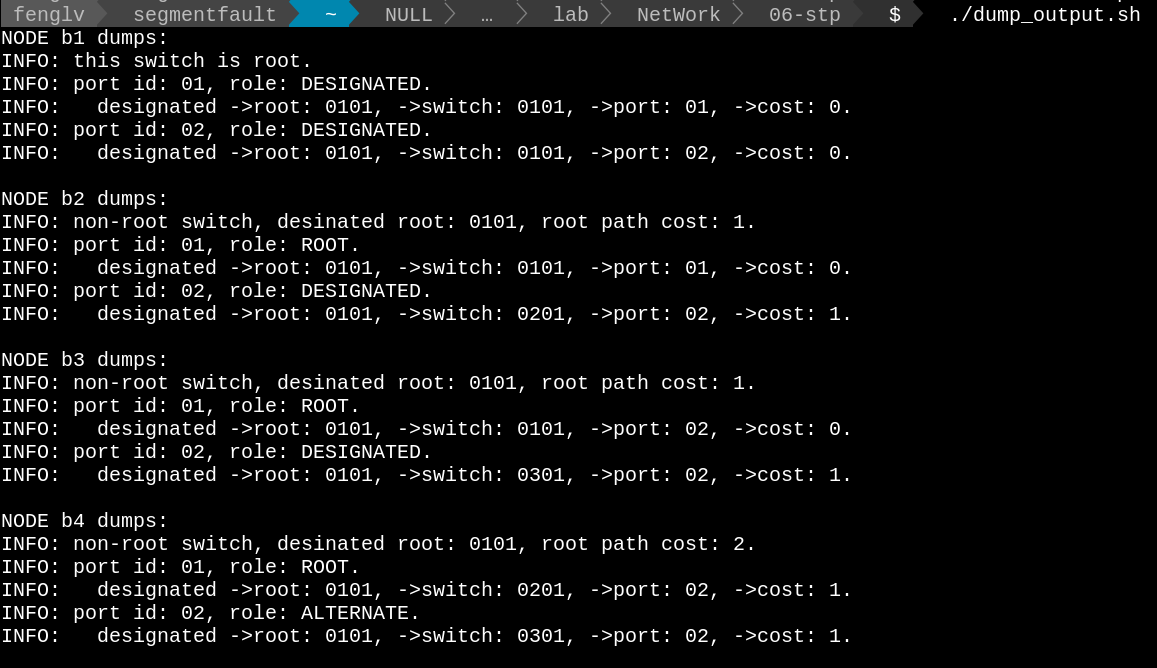
\includegraphics[scale=0.3]{./dump4.png}
  \caption{$dump$节点输出}
\end{figure}

使用新的更多节点和冗余链路的拓扑图进行实验,也能正确输出生成树拓扑。

\section*{{\CJKfamily{zhhei}结果分析}}
实验结果的正确性验证了生成树机制的正确性,通过不断发包收包,生成树能够在很快时间内形成并保存稳定。
\end{document}


